%%%%%%%%%%%%%%%%%%%%%%%%%%%%%%%%%%%%%%%%%
% Beamer Presentation
% LaTeX Template
% Version 1.0 (10/11/12)
%
% This template has been downloaded from:
% http://www.LaTeXTemplates.com
%
% License:
% CC BY-NC-SA 3.0 (http://creativecommons.org/licenses/by-nc-sa/3.0/)
%
%%%%%%%%%%%%%%%%%%%%%%%%%%%%%%%%%%%%%%%%%

%----------------------------------------------------------------------------------------
%	PACKAGES AND THEMES
%----------------------------------------------------------------------------------------

\documentclass{beamer}

\mode<presentation> {

%\usetheme{default}
%\usetheme{AnnArbor}
%\usetheme{Antibes}
%\usetheme{Bergen}
%\usetheme{Berkeley}
%\usetheme{Berlin}
%\usetheme{Boadilla}
%\usetheme{CambridgeUS}
%\usetheme{Copenhagen}
%\usetheme{Darmstadt}
%\usetheme{Dresden}
\usetheme{Frankfurt}
%\usetheme{Goettingen}
%\usetheme{Hannover}
%\usetheme{Ilmenau}
%\usetheme{JuanLesPins}
%\usetheme{Luebeck}
%\usetheme{Madrid}
%\usetheme{Malmoe}
%\usetheme{Marburg}
%\usetheme{Montpellier}
%\usetheme{PaloAlto}
%\usetheme{Pittsburgh}
%\usetheme{Rochester}
%\usetheme{Singapore}
%\usetheme{Szeged}
%\usetheme{Warsaw}

%\usecolortheme{albatross}
%\usecolortheme{beaver}
%\usecolortheme{beetle}
%\usecolortheme{crane}
%\usecolortheme{dolphin}
%\usecolortheme{dove}
%\usecolortheme{fly}
%\usecolortheme{lily}
%\usecolortheme{orchid}
%\usecolortheme{rose}
%\usecolortheme{seagull}
%\usecolortheme{seahorse}
%\usecolortheme{whale}
%\usecolortheme{wolverine}

%\setbeamertemplate{footline} % To remove the footer line in all slides uncomment this line
%\setbeamertemplate{footline}[page number] % To replace the footer line in all slides with a simple slide count uncomment this line

%\setbeamertemplate{navigation symbols}{} % To remove the navigation symbols from the bottom of all slides uncomment this line
}

\usepackage{graphicx} % Allows including images
\usepackage{booktabs} % Allows the use of \toprule, \midrule and \bottomrule in tables
\usepackage[spanish]{babel}
\usepackage[utf8]{inputenc}
\usepackage[T1]{fontenc}
\usepackage{textcomp}
\usepackage{geometry}
%\usepackage{movie15}
\usepackage{hyperref}

%----------------------------------------------------------------------------------------
%	TITLE PAGE
%----------------------------------------------------------------------------------------

\title[KiNAO]{Body Position and Orientation Recognition Library KiNAO} % The short title appears at the bottom of every slide, the full title is only on the title page

\author{Javier Acosta\\Daniel Méndez\\Willy Villalobos} % Your name
\institute[UCR] % Your institution as it will appear on the bottom of every slide, may be shorthand to save space
{
Universidad de Costa Rica \\ % Your institution for the title page
\medskip
\textit{} % Your email address
}
\date{\today} % Date, can be changed to a custom date

\begin{document}

	\begin{frame}
		\titlepage % Print the title page as the first slide
	\end{frame}

	\begin{frame}

		\begin{figure}
			\centering
			
\includegraphics[width=0.7\paperwidth,height=0.7\paperheight]{imagenes/KinaoNoBG.png}
		\end{figure}

	\end{frame}

%\begin{frame}
%\frametitle{Overview} % Table of contents slide, comment this block out to remove it
%\tableofcontents % Throughout your presentation, if you choose to use \section{} and \subsection{} commands, these will automatically be printed on this slide as an overview of your presentation
%\end{frame}

%----------------------------------------------------------------------------------------
%	PRESENTATION SLIDES
%----------------------------------------------------------------------------------------

%------------------------------------------------
%\section{First Section} % Sections can be created in order to organize your presentation into discrete blocks, all sections and subsections are automatically printed in the table of contents as an overview of the talk
%------------------------------------------------

%\subsection{Subsection Example} % A subsection can be created just before a set of slides with a common theme to further break down your presentation into chunks

%----------------------------------------------------------------------------------------
%----------------------------------------------------------------------------------------

	\begin{frame}
		\frametitle{¿Qué es KiNAO?}
		Es una librería que detecta el cuerpo humano, brindando datos sobre posición y orientación. La idea se  concibe como un paso para lograr controlar el movimiento de un robot NAO de forma que este replique las posiciones de una persona, utilizando un kinect como dispositivo de detección del movimiento.

		\begin{figure}
			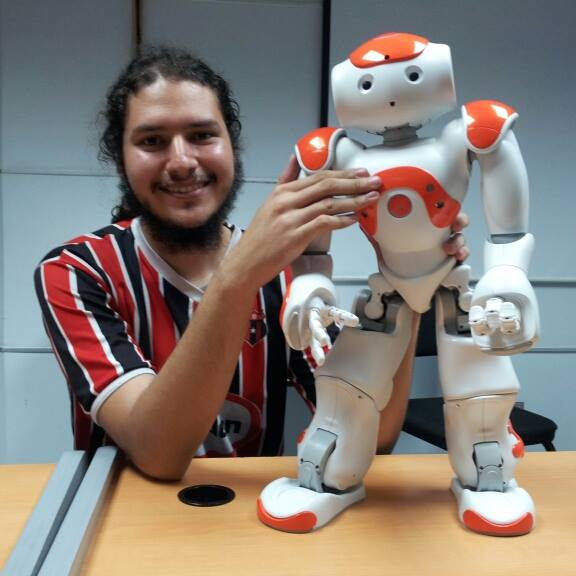
\includegraphics[width=0.4\linewidth]{imagenes/nao_and_me.jpg}
		\end{figure}

	\end{frame}
%----------------------------------------------------------------------------------------
	\begin{frame}
		\frametitle{¿Qué es KiNAO?}
		A partir de  la librería OpenNI se construyen los métodos adicionales necesarios para detectar el cuerpo y los movimientos, y posteriormente trasladar esa información al NAO para que la imite, o a cualquier autómata compatible, realizando la debida adaptación si fuese necesario.

		\begin{figure}
			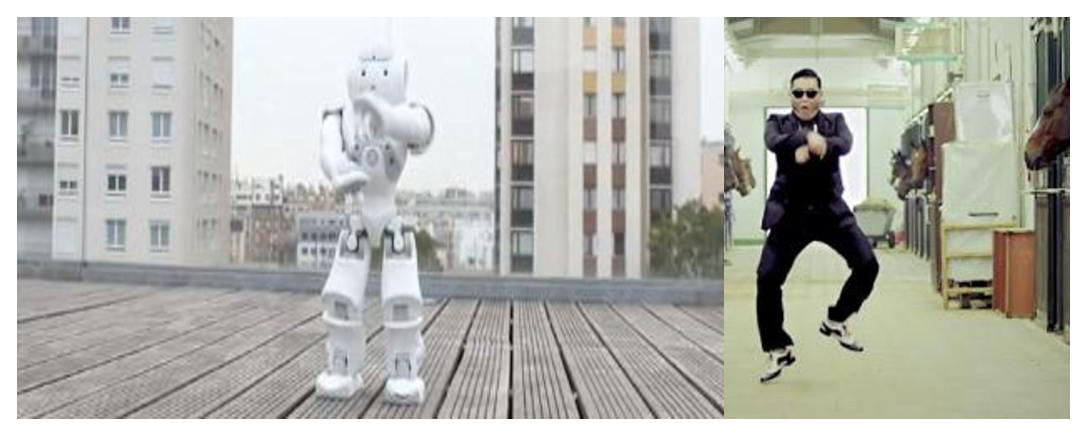
\includegraphics[width=0.7\linewidth]{imagenes/nao_gangnam.eps}
		\end{figure}

	\end{frame}
%----------------------------------------------------------------------------------------
	\begin{frame}
		\frametitle{Funcionamiento de la librería}
		Al momento de instalarse, OpenNI contiene una serie de archivos y librerías necesarios para la compilación y funcionamiento de los archivos, particularmente de los ejemplos de aplicación (samples) que incluye por defecto.

		\begin{figure}
			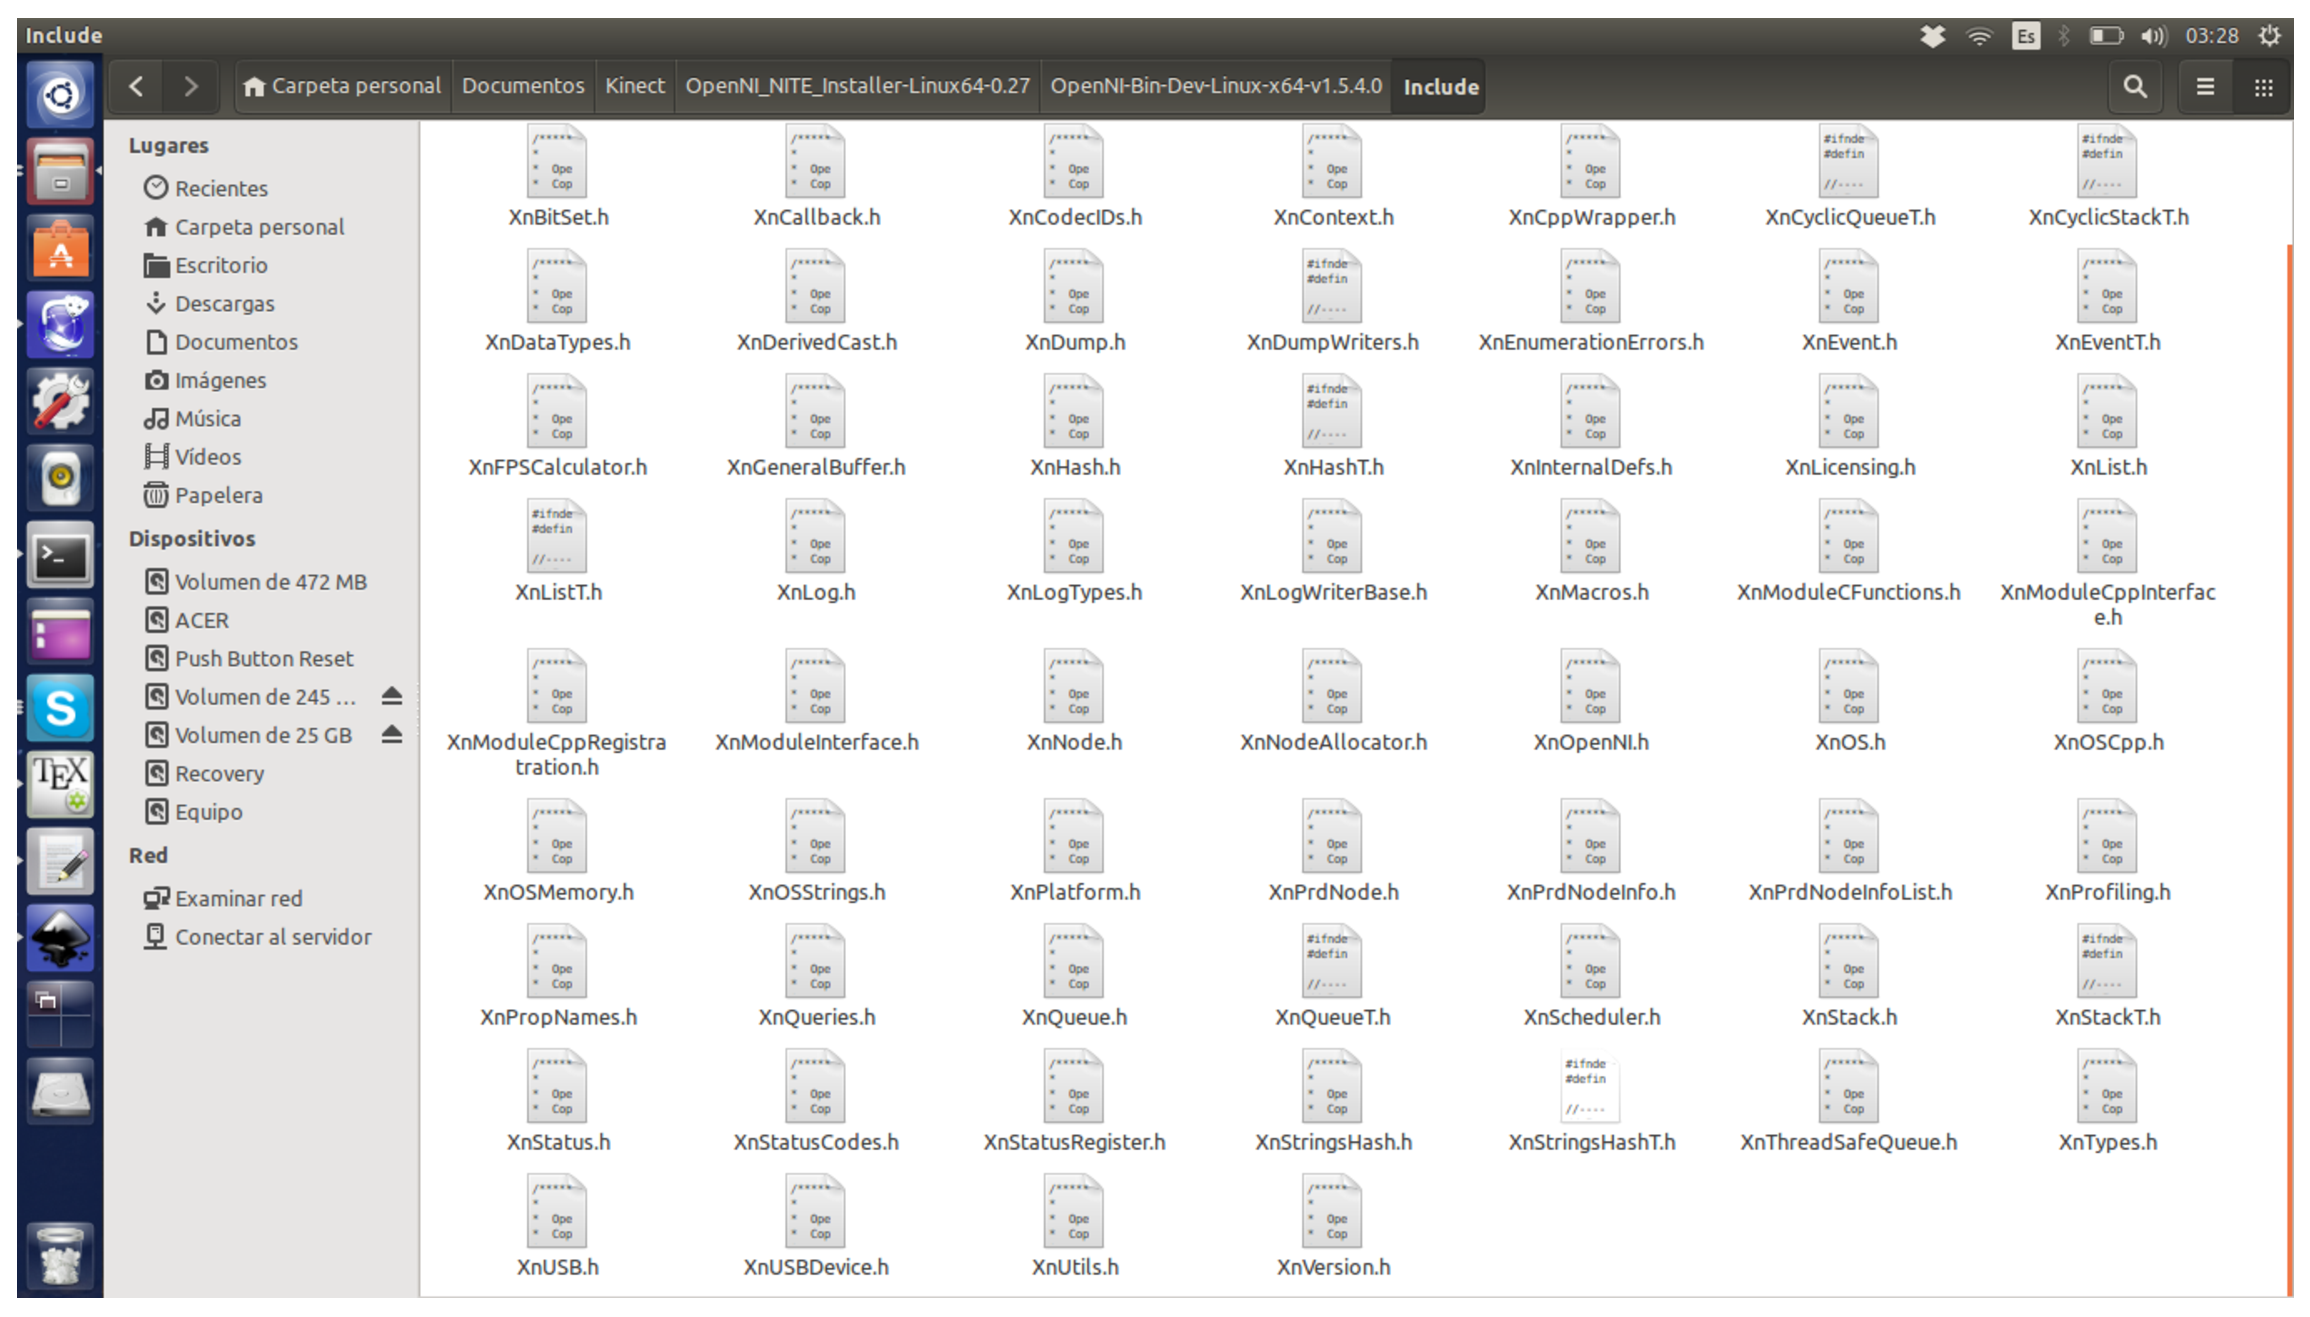
\includegraphics[width=0.7\linewidth]{imagenes/archivos_openni.eps}
		\end{figure}

	\end{frame}	%----------------------------------------------------------------------------------------
	\begin{frame}
		\frametitle{Funcionamiento de la librería}
		Para la librería desarrollada se tienen los siguientes archivos:

		\begin{enumerate}
			\item XnTypes.h
			\item definition.h
			\item XnCppWrapper.h	
			\item cpp\_global.h	
			\item kinao\_global.h
			\item joint.h
			\item joint.cpp
			\item larm.cpp (left arm), head.cpp...
		\end{enumerate}

	\end{frame}
%----------------------------------------------------------------------------------------
	\begin{frame}
		\frametitle{XnTypes.h}
		Este archivo define los tipos de datos necesarios para manipular toda la información que el kinect percibe, y que luego se procesa y despliega. 
	\end{frame}
%----------------------------------------------------------------------------------------
	\begin{frame}
		\frametitle{definition.h}
		Se definen nuevos tipos de datos necesarios para que los metodos de la nueva librería funcionen adecuadamente.
	\end{frame}
%----------------------------------------------------------------------------------------
	\begin{frame}
		\frametitle{XnCppWrapper.h}
		Esta librería contiene los métodos para calibración y reconocimiento del cuerpo, los samples de OpenNi se valen de esta librería, junto con otros archivos, para detectar a los usuarios y generar el "skeleton".
	\end{frame}
%----------------------------------------------------------------------------------------
	\begin{frame}
		\frametitle{cpp\_global.h}
		Este archivo se incluye únicamente en un eventual main para no tener que incluir por separado cada uno de los archivos de las partes del cuerpo que se van a reconocer con el kinect.
	\end{frame}
%----------------------------------------------------------------------------------------
	\begin{frame}
		\frametitle{kinao\_global.h}
		Este archivo se incluye en el joint.h ya que es la declaración de todas las clases y funciones de la librería. Al agregar nuevas librerías, se  deben incluir aquí por cuestiones de orden a la hora de programar.
	\end{frame}
%----------------------------------------------------------------------------------------
	\begin{frame}
		\frametitle{joint.h}
		Se realizan las definiciones de métodos y se heredan las clases necesarias para el funcionamiento de la librería.

		\begin{figure}
			\centering
			
\includegraphics[width=0.7\textwidth]{imagenes/doxygen.png}
		\end{figure}

	\end{frame}
%----------------------------------------------------------------------------------------
	\begin{frame}
		\frametitle{joint.cpp}
		Se declara la funcionalidad de la clase base joint.h y de los distintos métodos de la librería. Cada archivo de reconocimiento de estremidades, torso y cabeza emplea los métodos definidos en este archivo.

		\begin{figure}
			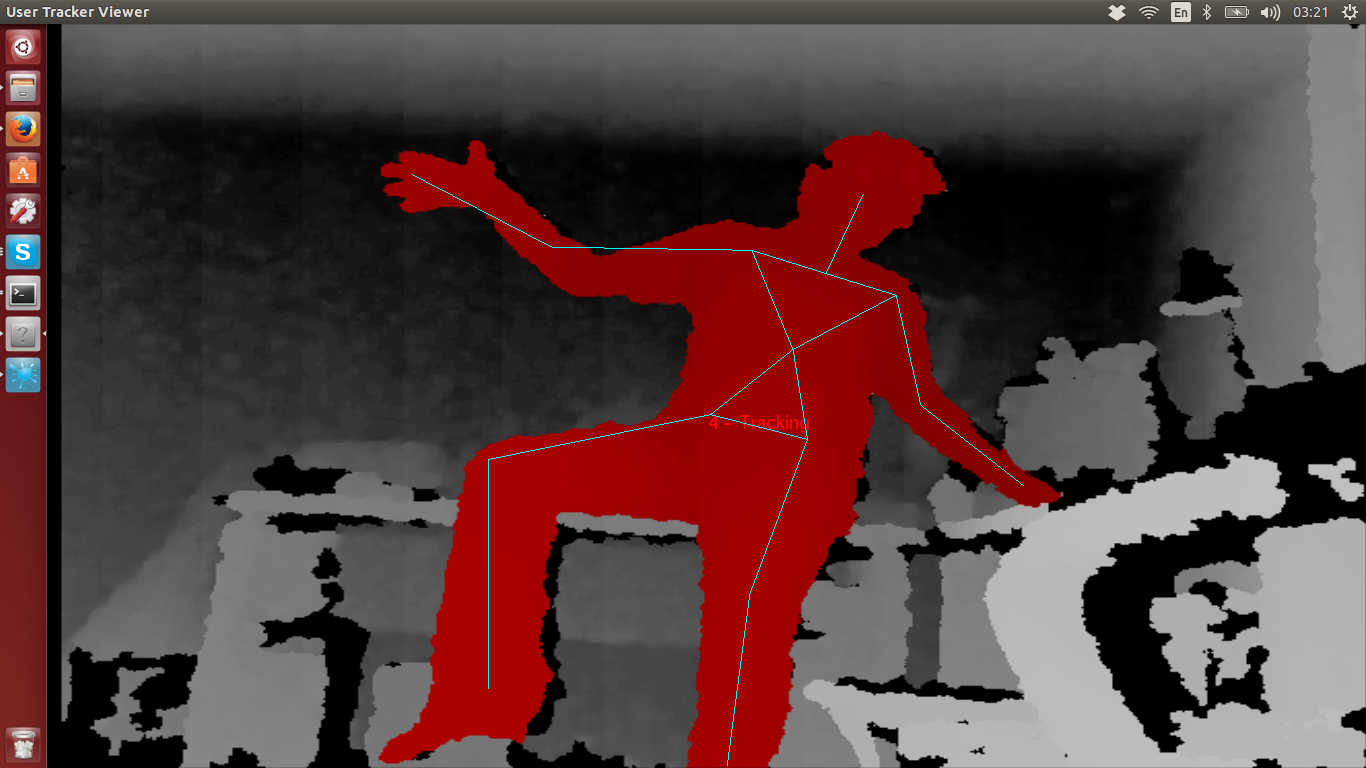
\includegraphics[width=0.7\linewidth]{imagenes/person.png}
		\end{figure}

	\end{frame}
%----------------------------------------------------------------------------------------
	\begin{frame}
		\frametitle{larm.cpp, head.cpp, ...}
		Estos  archivos aprovechan los métodos definidos en joint.h y joint.cpp para empezar a generar un esqueleto virtual de la persona detectada, e inclue métodos para obtener y procesar datos  de posición y orientación.
		\begin{figure}
			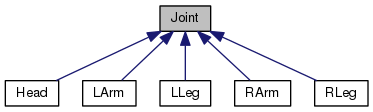
\includegraphics[width=0.6\linewidth]{imagenes/class_joint__inherit__graph.png}
		\end{figure}

	\end{frame}
%----------------------------------------------------------------------------------------
	\begin{frame}
		\frametitle{Tipos de datos importantes}
		Para la implementación de la librería se recurre a la definición de nuevos tipos de datos y de la reutilización de otros tipos de datos que por defecto define las librerías base del OpenNI. En este caso tenemos:

		\begin{enumerate}
			\item XnFloat
			\item XnVector3D
			\item XnReferenceAxis
		\end{enumerate}

	\end{frame}
%----------------------------------------------------------------------------------------
	\begin{frame}
		\frametitle{XnFloat}
		Es un tipo de dato que almacena un número con punto flotante, similar a float, para trabajar de forma aislada los datos e incluirlos más cómodamente en otras estructuras más complejas.
	\end{frame}
%----------------------------------------------------------------------------------------
	\begin{frame}
		\frametitle{XnVector3D}
		Es un tipo de dato  especial que genera un vector cuyas componentes son de tipo XnFloat definidas en el sistema de coordenadas rectangulares $(X,Y,Z)$

		\begin{figure}
			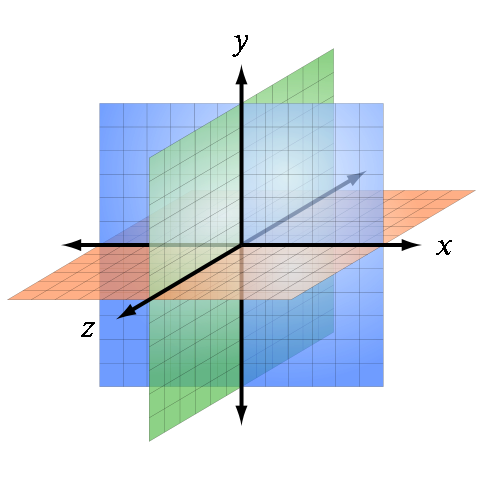
\includegraphics[width=0.55\linewidth]{imagenes/coordenadas.png}
		\end{figure}

	\end{frame}
%----------------------------------------------------------------------------------------
	\begin{frame}
		\frametitle{XnReferenceAxis}
		Este tipo de datos fue definido para efectos del proyecto, lo que hace es almacenar 3 vectores XnVector3D ortogonales entre si, formando un nuevo marco de referencia.

		\begin{figure}
			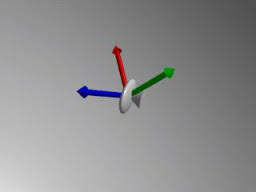
\includegraphics[width=0.55\linewidth]{imagenes/coordenadas-rotado.jpeg}
		\end{figure}

	\end{frame}
%----------------------------------------------------------------------------------------

%\begin{frame}
%\frametitle{Blocks of Highlighted Text}
%\begin{block}{Block 1}
%Lorem ipsum dolor sit amet, consectetur adipiscing elit. Integer lectus nisl, ultricies in feugiat rutrum, porttitor sit amet augue. Aliquam ut tortor mauris. Sed volutpat ante purus, quis accumsan dolor.
%\end{block}

%\begin{block}{Block 2}
%Pellentesque sed tellus purus. Class aptent taciti sociosqu ad litora torquent per conubia nostra, per inceptos himenaeos. Vestibulum quis magna at risus dictum tempor eu vitae velit.
%\end{block}

%\begin{block}{Block 3}
%Suspendisse tincidunt sagittis gravida. Curabitur condimentum, enim sed venenatis rutrum, ipsum neque consectetur orci, sed blandit justo nisi ac lacus.
%\end{block}
%\end{frame}

%------------------------------------------------

%\begin{frame}
%\frametitle{Multiple Columns}
%\begin{columns}[c] % The "c" option specifies centered vertical alignment while the "t" option is used for top vertical alignment

%\column{.45\textwidth} % Left column and width
%\textbf{Heading}
%\begin{enumerate}
%\item Statement
%\item Explanation
%\item Example
%\end{enumerate}

%\column{.5\textwidth} % Right column and width
%Lorem ipsum dolor sit amet, consectetur adipiscing elit. Integer lectus nisl, ultricies in feugiat rutrum, porttitor sit amet augue. Aliquam ut tortor mauris. Sed volutpat ante purus, quis accumsan dolor.

%\end{columns}
%\end{frame}

%------------------------------------------------
%\section{Second Section}
%------------------------------------------------

%\begin{frame}
%\frametitle{Table}
%\begin{table}
%\begin{tabular}{l l l}
%\toprule
%\textbf{Treatments} & \textbf{Response 1} & \textbf{Response 2}\\
%\midrule
%Treatment 1 & 0.0003262 & 0.562 \\
%Treatment 2 & 0.0015681 & 0.910 \\
%Treatment 3 & 0.0009271 & 0.296 \\
%\bottomrule
%\end{tabular}
%\caption{Table caption}
%\end{table}
%\end{frame}

%------------------------------------------------

%\begin{frame}
%\frametitle{Theorem}
%\begin{theorem}[Mass--energy equivalence]
%$E = mc^2$
%\end{theorem}
%\end{frame}

%------------------------------------------------

%\begin{frame}[fragile] % Need to use the fragile option when verbatim is used in the slide
%\frametitle{Verbatim}
%\begin{example}[Theorem Slide Code]
%\begin{verbatim}
%\begin{frame}
%\frametitle{Theorem}
%\begin{theorem}[Mass--energy equivalence]
%$E = mc^2$
%\end{theorem}
%\end{frame}\end{verbatim}
%\end{example}
%\end{frame}

%------------------------------------------------

%\begin{frame}
%\frametitle{Figure}
%Uncomment the code on this slide to include your own image from the same directory as the template .TeX file.
%\begin{figure}
%
\includegraphics[width=0.8\linewidth]{test}
%\end{figure}
%\end{frame}

%------------------------------------------------

%\begin{frame}[fragile] % Need to use the fragile option when verbatim is used in the slide
%\frametitle{Citation}
%An example of the \verb|\cite| command to cite within the presentation:\\~

%This statement requires citation \cite{p1}.
%\end{frame}

%------------------------------------------------

%\begin{frame}
%\frametitle{References}
%\footnotesize{
%\begin{thebibliography}{99} % Beamer does not support BibTeX so references must be inserted manually as below
%\bibitem[Smith, 2012]{p1} John Smith (2012)
%\newblock Title of the publication
%\newblock \emph{Journal Name} 12(3), 45 -- 678.
%\end{thebibliography}
%}
%\end{frame}

%------------------------------------------------
	\begin{frame}
		\Huge{\centerline{Tiempo para una demostración}}

		\begin{figure}
			\centering
			
\includegraphics[width=0.4\paperwidth,height=0.4\paperheight]{imagenes/KinaoNoBG.png}
		\end{figure}

	\end{frame}
%----------------------------------------------------------------------------------------
	\begin{frame}
		\Huge{\centerline{Gracias por su atención}}
	\end{frame}
%----------------------------------------------------------------------------------------

\end{document} 
